%%
\chapter{Generating query based monitoring components}
%%

After the domain model of the system is designed, and the graph queries are written, the monitoring components can be generated and deployed along with \cpp{} tools for modeling the domain.
As stated before, domain modeling and graph query definition are done using EMF and \viatra{} technologies.
In this chapter, I present how the monitoring components are generated from these artifacts.

From the metamodel, the framework generates the classes, which enables the programmer to model the system's state in \cpp{}.
Also, we generate the monitoring code for the system, which is basically the \cpp{} implementation of the planned graph queries. 
These graph queries are evaluated on the maintained \cpp{} model at runtime, to show if there are some problems in the system.

%%%%
%%%%
%%%%
		\section{Generating classes from the metamodel}
%%%%
%%%%
%%%%

The domain model consists of packages (EPackage), enumerations (EEnum) and classes (EClass).
From an EPackage, we generate a folder; Every source file originated from an elements from the package will be generated in that folder. 
We generate sources from each class and enumeration of the package, also we generate other artifacts for the package, like helper classes, or model handling tools.


\subsection{Mapping an EClass to \protect\cpp }


\todo{ábra szépítés}
\begin{figure}
	\begin{center}
		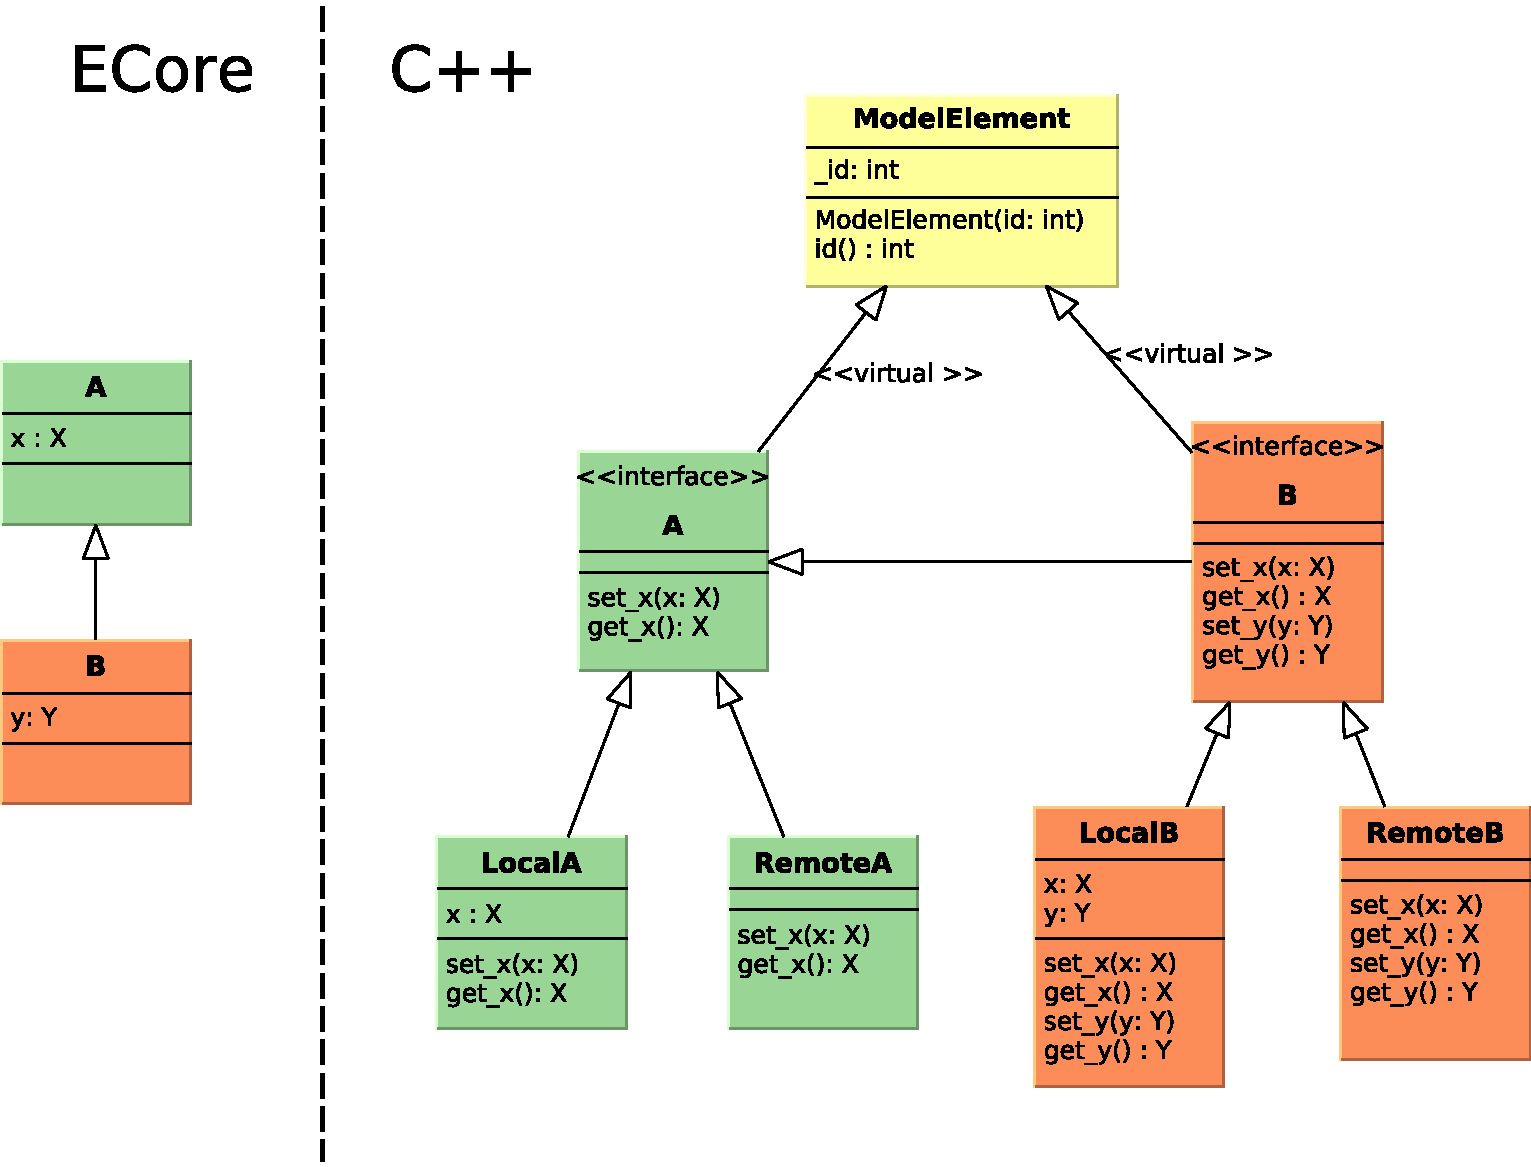
\includegraphics[width=\textwidth]{figures/eclass-to-cpp.pdf}
		\caption{Mapping of two EClasses, one inherited from the other (Left: EClasses, right: \protect\cpp{} classes) }
		\label{fig:eclass-to-cpp}
	\end{center}
\end{figure}


The EClasses of the metamodel are mapped to various \cpp{} classes, as depicted on \mbox{Figure~\ref{fig:eclass-to-cpp}}.
From each EClass we generate three \cpp{} classes:

\begin{itemize}
	\item An interface (abstract class with only pure virtual methods in \cpp{})
	\item A local class
	\item A remote class
\end{itemize}


The interface provides access to an instance of the EClass.
The local class implements the interface. It stores the attributes and references of the instances allocated to the local computing unit, and made them accessible by the methods of the implemented interface.
The remote class implements the interface, but are only used to substitute remote objects in references to them; 
Accessing its variables are not possible, because they are stored in another node. 

\subsection{Mapping an EEnum to \protect\cpp }

Enumerations are simply mapped to \cpp{} enum classes as depicted on Fig.\ref{fig:eenum-to-cpp}.

\begin{figure}[H]
	\begin{center}
		
		\begin{minipage}[c]{\textwidth}
		\begin{minipage}[r]{0.52\textwidth}
			\hfill
			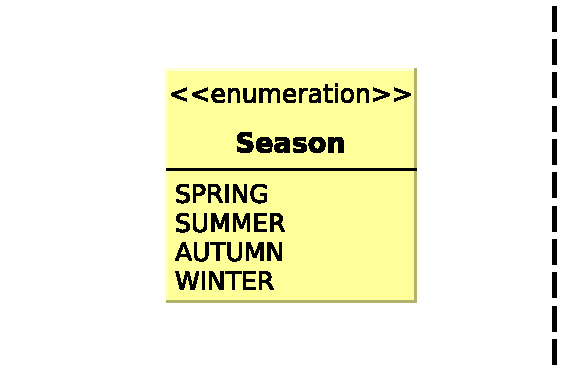
\includegraphics[width=0.735\textwidth]{figures/eenum-to-cpp.pdf}
		\end{minipage}
			\hspace{0.05\textwidth}
		\begin{minipage}[c]{0.25\textwidth}
\begin{lstlisting}[language=C++]
namespace Package{

enum class Season{
	SPRING = 0,
	SUMMER = 1,
	AUTUMN = 2,
	WINTER = 3
};

}
\end{lstlisting}			
		\end{minipage}
		\end{minipage}
		\caption{Mapping of an enumeration to \protect\cpp{} enum class }
		\label{fig:eenum-to-cpp}
	\end{center}
\end{figure}

\subsection{ Generating ModelRoot class }

A class called ModelRoot is also generated.
The purpose of ModelRoot is to handle the whole model of the system: 
It contains the instances of the classes and it keeps track of the objects by identifier.
It also provides a method to read in initial models from a json file.
The ModelRoot class is also the connection point between the monitoring components and the model.

\subsection{ Other sources }

For each package the framework generates
\begin{itemize}
	\item a header file containing forward declarations for each generated classes
	\item a header file including all the full declaration of classes
	\item a header file containing string conversion methods for enumerations, as \cpp{} lacks this feature in enum classes.
\end{itemize} 



%%%%
%%%%
%%%%
		\section{Overview of the query compilation workflow}
%%%%
%%%%
%%%%



The compilation of the queries of the CPS is depicted in fig. \ref{figure:query-compile-workflow}. 
First, vql files are parsed using EMF so their contents are loaded into a Pattern Model.
The Pattern Model are processed by \viatra{} and converted into PSystem representation of queries.
After that, we extend this representation with type information, as type information is more important in the \cpp{} generated code, than in the \viatra implementation of local search.
Then, we create the plan for query execution; We use the local search planner of \viatra{} fine tuned with our search operation cost function to improve performance of distributed queries. 
We also use some optimizations later to improve distributed performance. 
After the fully optimized plan is ready, we can construct the generator model describing the source code structure and generate the \cpp{} files.


\begin{figure}[h]
	\begin{center}
		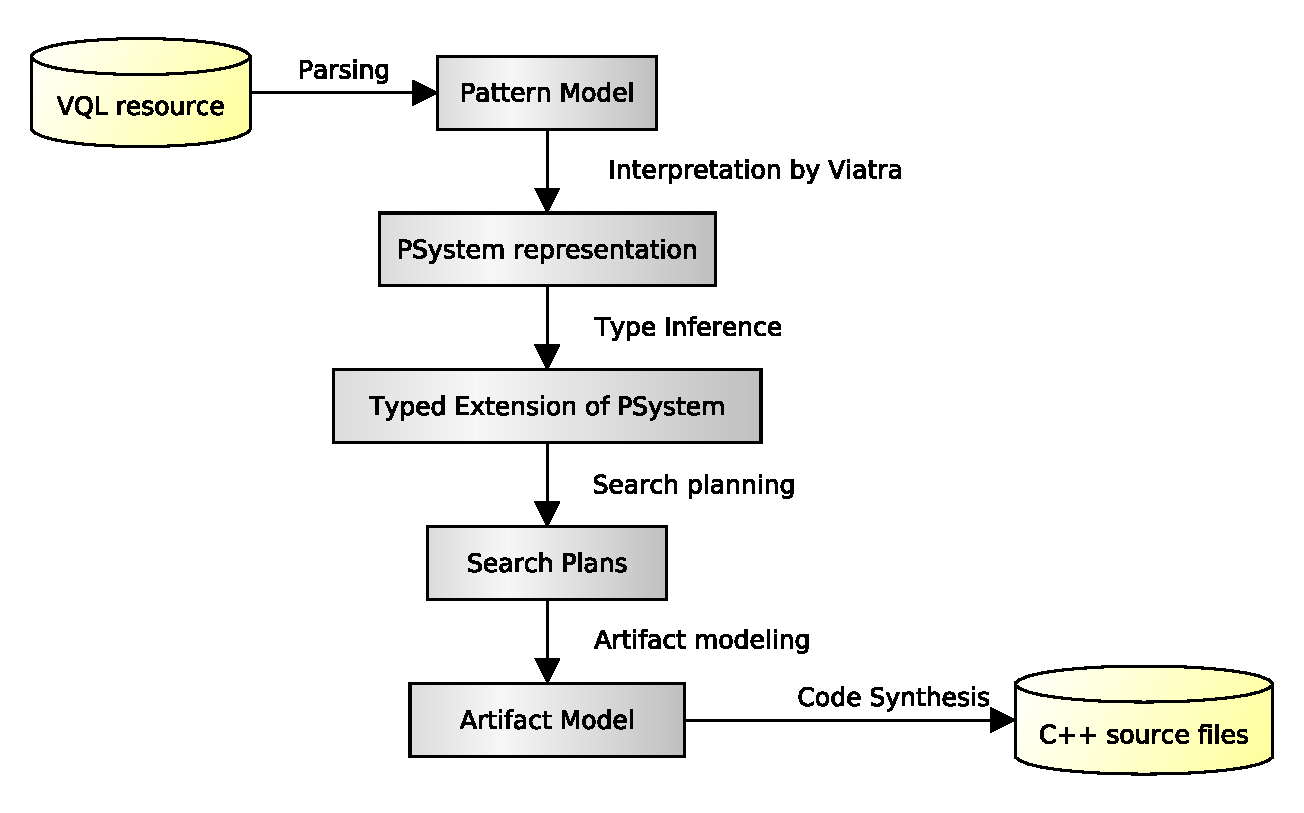
\includegraphics[width=0.8\textwidth]{figures/query-compilation-workflow.pdf}
		\caption{Query compilation workflow}
		\label{figure:query-compile-workflow}
	\end{center}
\end{figure}



\subsection{PSystem representation}


The vql file is loaded into a PatternModel, which is a model for vql files. 
The framework does not use this representation, but passes it to \viatra, which creates its own representations of it called PSystem. \cite{psystem}. 


\begin{figure}
	\begin{center}
		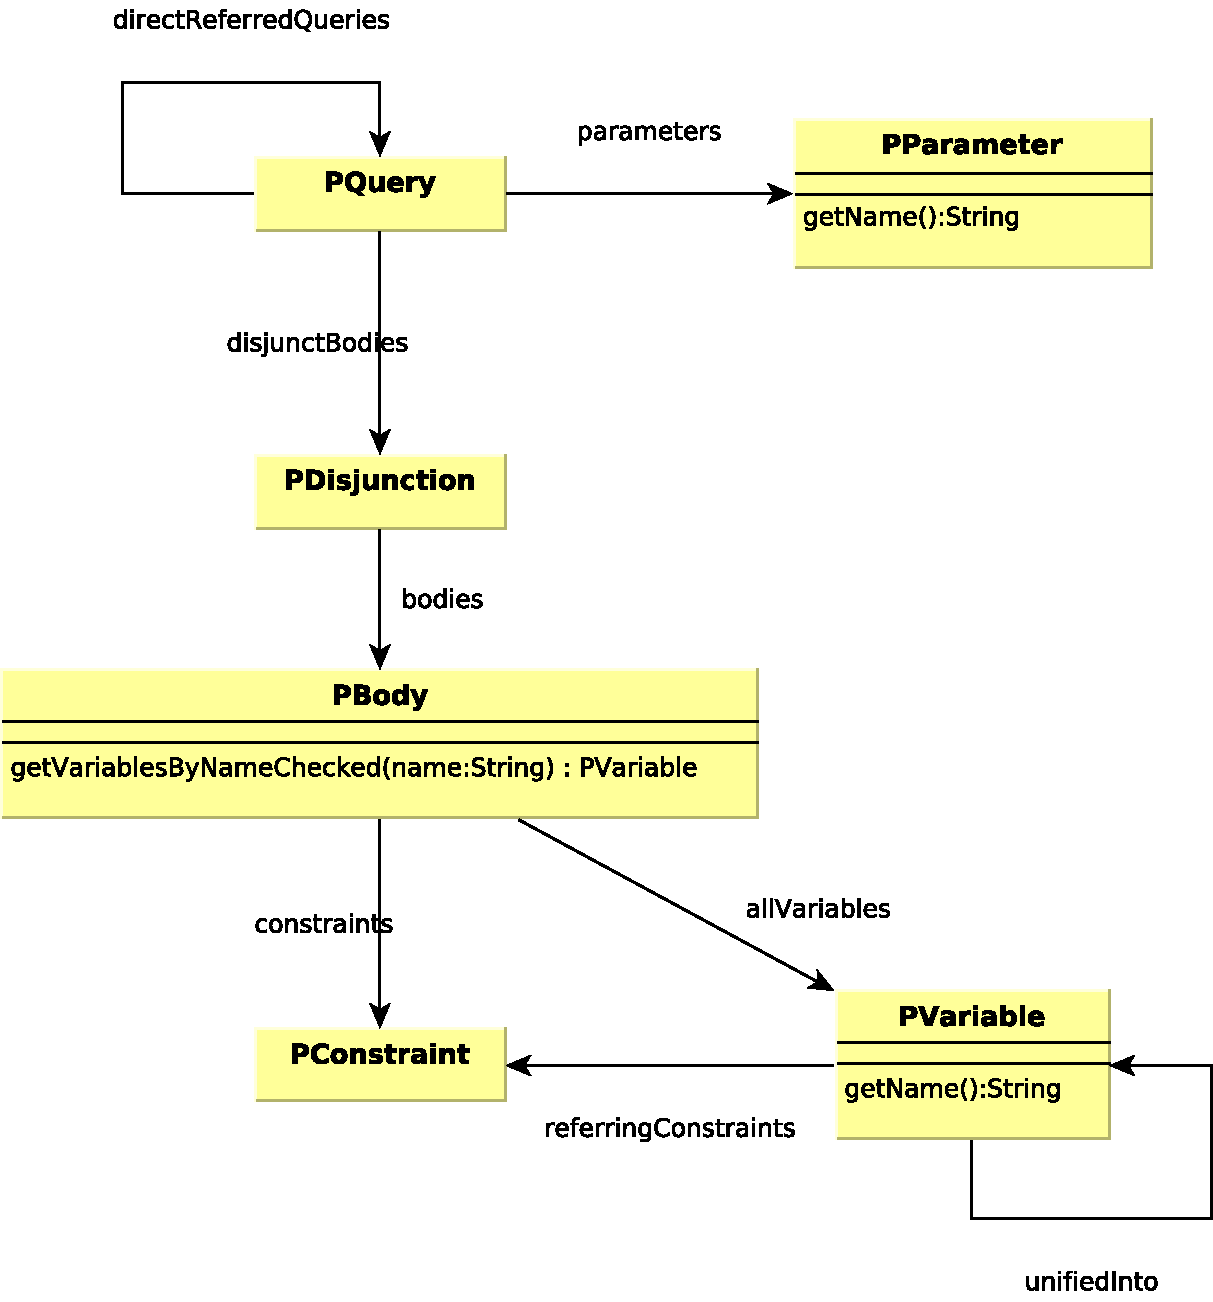
\includegraphics[width=0.6\textwidth]{figures/psystem.pdf}
		\caption{PSystem's structure}
		\label{fig:psystem}
	\end{center}
\end{figure}
The structure of PSystem representation is shown on Figure~\ref{fig:psystem}. 
As their implementation is hidden behind interfaces, most of the refrences means getter functions (In Xtend, gettern functions can be used with field access syntax like \csharp{} properties). 
Graph patterns are represented by a PQuery. 
A PQuery has a parameter list. 
The most important attribute of parameters are its names. 
A PQuery consists of a PDisjunction, which consists of a set of PBodies. 
PDisjunctions play role in Query rewriting, where the bodies of a PQuery gets optimized, or changed other ways.
PBody consists of PConstraints. 
PConstraint is a basic interface for various constraints. 
Altough constraints refer to variables, all variablesin a PBody can be accessed from PBody.

A variable can be unified into another variable. 
This can happen when equality constraint is used between two variable: 
Equality constraint is omitted, one of the variable gets unified into the other, and other constraints do not have to be changed.

%TODO Az ábra még pontosítható
\todo{ Az ábra még pontosítható}


\subsection{Typed Extension of PSystem}

To make PSystem more usable we extend it with additional information, mainly with type information for variables and parameters.
For this the types of the variables and parameters must be infered based on type constraints of the graph pattern.

First the types of the variables must be infered. 
First, we collect all the type constraints, that the variable must satisfy.
We do this, by collecting all the variables that are the same as the variable( via equality constraint eg. ), 
then collect the constraints refering to them.
From this we can create a set of candidate types.
Then we choose the type as the following. 
If the types contains classes and datatypes, then we throw an error.
If all the types are data types, then they must be compatible with each other (integral types, or the same type).
In this case, the most specific is choosen. If there are uncompatible types, then we throw an error.
If all the types are EClass types, then we select the most general class, that are compatible (extends it or is the same) of all the classes and choose that.
If we cannot choose such EClass, or there are multiple classes that satisfies this, then we throw an error (The later can happen eg., when there are two classes, A and B, and exists two class, that are a descendant of both of them).


\begin{figure}[h]
	\begin{center}
		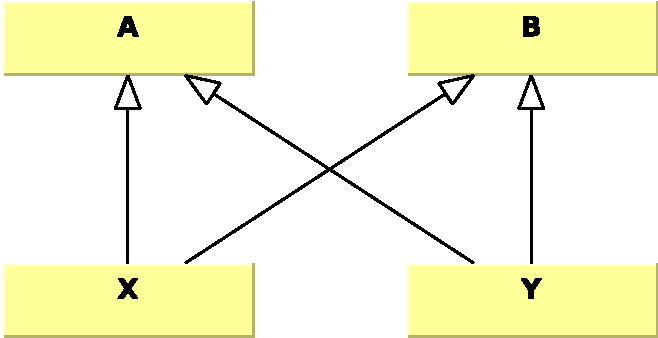
\includegraphics[width=0.4\textwidth]{figures/multiple-inheritance-problem.pdf}
		\caption{Problems with type inference in case of multiple inheritance}
		\label{fig:multiple-inheritance-problem}
	\end{center}
\end{figure}

If the types of the variables are known then the types of the parameters can be infered. 
For this, we collect the variables that represents this parameter from each body.
As the parameters value can be any of the variable, we choose the type, that generalizes them.

We also maintain additional information in our representation. 
Bodies also maintain the relationship between variables and parameters. 
In PSystem, this information is not directly available, parameters and variables need to be matched by name.

\subsection{Search planning}

After we have extended PSystem with the needed information, we can plan how the pattern will be executed.
From a set of constraints that declaratively defines the pattern we need to create an imperative sequence of search operations.

For this, we use the local search planner of \viatra{}.
This planner takes a cost function, then creates a permutation of constraints that minimizes the cost function. 
After this permutation is achieved, then search operations will be created by mapping the constraints to them considering their position.
The cost function must give an approximated cost of applying a constraint based on the variables bound before the application and other information (Like statistics on the instance model, that can only be available at runtime, so \viatra{} can utilize them, but we can't as we generate the monitoring components at design time). 

For the different constraint applications we use the following search operations.

\subsubsection{Type constraint}
If a variable must be of a given type, then the following two search operation can be the next:
If the variable is bound, we need to check wether the already bound value is of that type, we denote this CheckInstanceOf(Var, Type).
If the variable is unbound, we need to iterate over the instances of the type and follow the algorithm, we denote this ExtendInstanceOf(Var, Type) ).


\subsubsection{Reference and attribute constraint}

If a structural feature is \todo{befejezni innentől ezt a fejezetet}


\subsubsection{Negative pattern application}


\subsubsection{Transitive closure}





\subsection{Additional optimization}

After we complete the plan with type information and other details, it can be used to generate C++ code, although before that step we use further optimizations. 
These optimizations considers distributed execution of the plan, so it can improve the plan generated by \viatra{} which is generated to be used in a single computer.


\subsubsection{Replace pattern calls with simpler operations}
There are some cases, where helper patterns are simple, and used to define simple conditions. 
In this case, evaluationg the subquery is not always the most efficient method, sometimes these can be replaced by simple search operations:

\subparagraph{Reference Pattern}
We use the phrase \emph{reference pattern} for a pattern with 2 parameters if its only constraint is that a reference exist between the two parameters, eg.:
\begin{lstlisting}[language = vql]
private pattern connected(a : RailRoadElement, b : RailRoadElement){
	RailRoadElement.connectedTo(a,b);
}
\end{lstlisting}

In the following examples i will use this query as an example to demonstrate how the application of this query can be replaced by an other operation.

\subparagraph{Counting reference pattern} 

\begin{lstlisting}[language = vql]
1 == count find connected(a, _);
\end{lstlisting}


\subparagraph{Negative application of a reference pattern}

\begin{lstlisting}[language = vql]
neg find connected(a, _);
\end{lstlisting}

\subsubsection{Filter unnecessary operations, checks}
As the original plan is generated by the localsearch planner of \viatra{}, there can be redundant operations, which can be ommited. This includes:

\begin{itemize}
	\item Check operation -- The generated code is strongly typed, so we don't need type checks in most cases, unlike in the Java implementation, where the tuples contains plain java objects with unknown types.
	
	\item Distribution operations -- \todo{KIFEJTENI}
\end{itemize}



\subsection{C++ code generation}

The completed and optimized plan are used to generate \cpp{} code. 
Two main methods can be used to run local search plan in case of generated code. 
One is to generate the plan as a data structure and create an interpreter that uses that plan to find matches. 
The other is to generate the code directly from the plan. 
The first method is good if we want to change the plan at runtime, but the interpreter itself introduces an overhead, causing performance to be slower.
We used the later, because we don't change the plan at runtime.












